\chapter{基于GPU的极大二分团枚举并行实现}
\label{ch:gmbe}

针对现有极大二分团枚举算法在并行扩展性方面受限于CPU计算核心数量的问题,本章引入了具有大量计算核心的GPU作为计算资源,以加速极大二分团枚举过程。本章介绍了现代GPU的硬件架构和软件编程模型。同时,本章%整理了GPU加速图计算的相关工作,并
指出在GPU上实现极大二分团枚举所面临的挑战,作为研究的动机。具体而言,简单地将现有算法映射到大量的GPU计算核心中会遇到内存短缺、线程分歧和负载不均等问题。为了解决这些问题,本章提出了以下优化方法:首先,针对内存短缺问题,本章提出了基于节点重用的迭代计算流程。该方法可以重用枚举树根节点内存,避免为新枚举节点动态分配内存,从而减少内存开销。其次,针对线程分歧问题,本章提出了基于局部邻居数量感知的剪枝方法。该方法通过记录枚举过程中顶点局部邻居数量的变化对枚举空间进行剪枝,缓解了线程分歧问题。然后,针对负载不均问题,本章提出了负载感知的任务调度方法。该方法将每颗子枚举树对应的计算任务与一个线程束的计算资源进行绑定,在运行时动态预估子枚举树的大小并对较大的子枚举树进行进一步拆分,实现了细粒度的负载均衡。最后,本章结合上述三种方法,提出了基于GPU的高效极大二分团枚举解决方案GMBE。实验证明,基于单个NVIDIA A100 GPU的GMBE相比现有基于96个CPU的并行算法parMBE实现了70.6倍的性能提升。

\section{现代GPU架构与编程模型} 
GPU,即图形处理单元(Graphics Processing Unit),最初是专门用于处理图形数据的处理器。随着计算需求的增加,现代GPU逐渐演变成了通用并行处理器,能够高效执行大规模数据并行计算任务,如科学计算、深度学习和密码学等。与传统的中央处理器(central processing unit, CPU)相比,现代GPU拥有更多的计算核心,并且能够利用这些核心并行处理大量数据,因此成为加速图计算的有力工具,同时具备加速极大二分团枚举问题的潜力。在本节中,我们将深入探讨现代GPU的硬件架构、与硬件架构对应的主流的软件编程模型CUDA (compute unified device architecture)以及针对CUDA的编程指南,作为本章的研究背景。

\begin{figure} [t]
  \center
    \vspace{0.1in}
		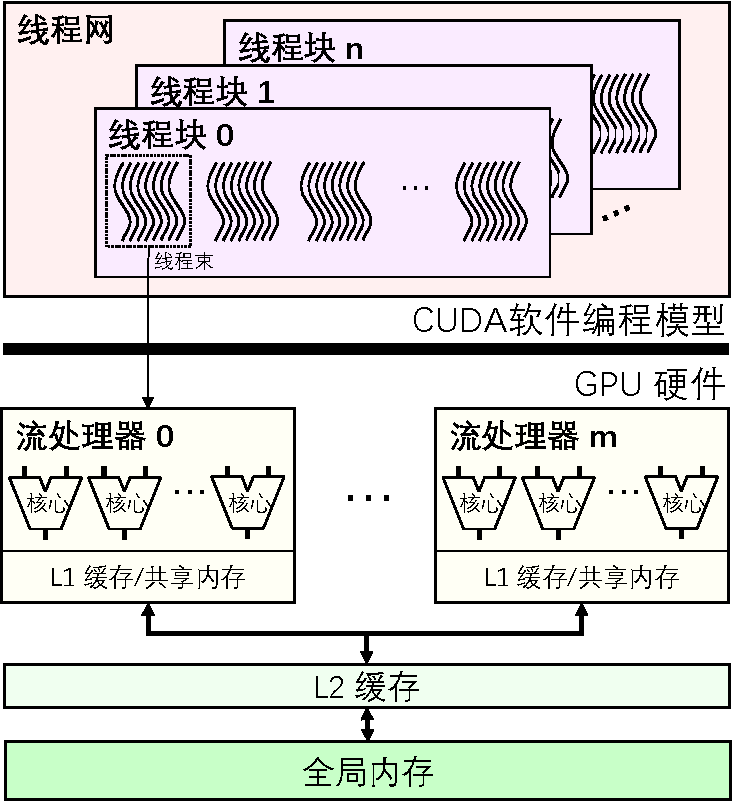
\includegraphics[width=0.55\linewidth]{gpu_arch}
    \vspace{0.1in}
	\caption{现代GPU硬件架构与软件编程模型}
	\label{fig:gpu}
\end{figure}

图\ref{fig:gpu}展示了现代GPU的硬件架构和软件编程模型。GPU的\textbf{硬件架构}包括大量的计算核心,以及对应的层级存储结构。具体而言,一块现代GPU通常包括全局内存(global memory)、共享的L2缓存(cache)以及大量的流处理器 (streaming multiprocessor, SM)。每个流处理器包含单独的L1缓存、可编程的具有多分区(multi-bank)的共享内存(shared memory),以及多个轻量级计算核心(core)。主流的GPU可以配备上万个轻量级计算核心,提供了巨大的计算能力。然而,与丰富的计算资源相比,GPU上的内存资源相对有限。例如,近年备受青睐的NVIDIA A100~\cite{NVIDIA-A100}最多可以提供6912个核心,但只能提供最多80GB的全局内存。

与GPU的多计算核心的硬件架构相对应,主流的\textbf{CUDA软件编程模型}按照层级结构管理大量线程。具体而言,CUDA编程模型提供了一个并行计算平台和一组API~\cite{CUDA-wiki,CUDAProgrammingGuide},允许用户高效地利用GPU进行通用目的的处理。CUDA采用SIMT (single instruction, multiple threads)~\cite{SIMT-wiki} 执行模型来管理大量线程。它将GPU内核划分为多个网格 (grid),每个网格包含多个块 (block),每个块包括多个线程 (thread),并在执行期间分配给一个流处理器 (SM)。流处理器将32个并行线程分组成一个线程束 (warp),并同时执行多个线程束。通过这种方式,成千上万个GPU核心可以高效地并行工作,实现高性能计算。

为了提升GPU的执行性效率,我们针对CUDA编程模型总结了\textbf{编程指南}如下:

\begin{enumerate}
  \item 减少动态内存分配。动态内存分配是指程序在运行过程中动态申请和释放内存。由于 GPU 允许大量的线程同时并发执行,大量线程可能会同时进行动态内存分配,从而引发线程争用、同步开销和内存碎片化等问题 ~\cite{DynamicMallocGpu21}。为了避免这种情况的发生,建议采用预分配内存等方式减少动态内存分配,以降低内存管理的开销并优化内存访问效率。
  
  \item 减少线程分歧。线程分歧是指在 GPU 中同一线程束内的线程执行不同的代码路径。由于 GPU 使用 SIMT 的执行模式,即多个线程共享同一组指令,线程分歧会使 GPU 对不同执行路径进行串行化,从而严重影响执行性能 ~\cite{CUDAProgrammingGuide}。因此,在程序设计时应尽量最小化条件分支语句的使用,确保同一线程束的线程能执行相同的代码路径,从而提高并行执行效率。

  \item 平衡大量负载。负载均衡是指将计算任务平均分配给 GPU 不同的计算资源。由于 GPU 拥有大量轻量级计算核心,负载不平衡会导致数千个计算核心等待最慢的计算核心执行,造成严重的资源浪费~\cite{CUDAProgrammingGuide}。为了解决这一问题,建议在程序设计时使用动态任务分配方法,以实现计算任务在不同计算资源上的均匀分布,从而提高整体计算效率。
\end{enumerate}


\section{研究动机}

尽管GPU具有强大的并行能力,在部分图挖掘问题上已经显示出加速效果,但在GPU上实现高效的极大二分团枚举仍然面临严峻的挑战。具体而言,这些挑战主要包括内存短缺、线程分歧和负载不均等。本节将结合GPU加速图计算的相关工作,对上述挑战进行详细说明。
\subsection{内存短缺}

\subsection{线程分歧}

\subsection{负载不均}


\section{GMBE算法设计与实现}

\subsection{基于节点重用的迭代计算流程}

\subsection{基于局部邻居数量感知的剪枝方法}

\subsection{负载感知的任务调度方法}

\subsection{GMBE算法}

\section{实验评估}

\subsection{实验设置}

\subsection{整体评估}

\subsection{细分评估}

\subsection{敏感性测试}

\section{本章小结}